\thispagestyle{plain}
\section{Results}
\label{sec:results}

This section presents the empirical findings from the carbon emission forecasting models developed according to the methodology outlined in the previous section. The analysis unfolds systematically to evaluate both forecasting performance and findings across the prediction horizons.

Baseline model results establish the performance thresholds that the long short-term memory neural network (LSTM) architectures must exceed to demonstrate value. The investigation then advances through the LSTM implementations, examining hyperparameter optimization and training dynamics for both 1-hour and 24-hour forecasting tasks. Beyond predictive accuracy, the analysis dives deeper into the 24-hour LSTM through feature importance analysis, revealing which variables drive forecasting performance and validating the theoretical foundations underlying variable selection. Note that all error figures, such as Root Mean Squared Error (RMSE) and Mean Absolute Error (MAE), are reported in tonnes \cotwoe{} unless otherwise stated.

\subsection{Baseline Model Performance}

Four baseline models were established to provide comparative benchmarks for evaluating LSTM performance across both forecasting horizons. The naive persistence models assume that future carbon emissions equal the most recent observed value, implemented as \(\hat{y}^{(t+1)} = y^{(t)}\) for the 1-hour horizon and \(\hat{y}^{(t+h)} = y^{(t)}\) for \(h \in \{1, 2, \ldots, 24\}\) in the 24-hour forecasting task.

For the ARIMA models, systematic grid search optimization was conducted across all parameter combinations as specified in the methodology. The optimal configuration for both forecasting horizons was identified as ARIMA(5,0,5) with no trend component, indicating that an autoregressive order of 5, no differencing, and a moving average order of 5 provided the best out-of-sample validation performance for both the 1-hour and 24-hour prediction tasks.

The final test set evaluation revealed substantial performance differences across models and forecasting horizons. For the 1-hour ahead forecasting task, the naive persistence model achieved a test RMSE of 10.54 and MAE of 6.13, while the ARIMA(5,0,5) model demonstrated improved performance with an RMSE of 9.43 and MAE of 5.99. The 24-hour forecasting horizon presented considerably greater prediction complexity, with the naive persistence model yielding a test RMSE of 29.75 and MAE of 20.33, and the ARIMA(5,0,5) model achieving an RMSE of 25.03 and MAE of 18.21.

To validate the statistical significance of these performance differences, two-sided Diebold-Mariano tests were conducted comparing ARIMA against naive persistence models for both forecasting horizons. The tests confirmed statistically significant improvements, with p-values effectively zero for both the 1-hour (DM statistic: -12.12) and 24-hour (DM statistic: -16.15) comparisons, enabling rejection of the null hypothesis of equal predictive accuracy at the \(\alpha = 0.05\) significance level.

The consistent pattern of ARIMA outperforming naive persistence across both RMSE and MAE metrics, validated through statistical testing, confirms the value of capturing linear temporal dependencies in carbon emission patterns. However, the substantial increase in error magnitudes from 1-hour to 24-hour forecasting horizons across both evaluation metrics underscores the inherent difficulty of extended prediction periods in volatile wind power grids. These baseline results establish the performance thresholds that the LSTM architectures must exceed to demonstrate meaningful forecasting improvements.

\subsection{LSTM Hyperparameter Optimization and Training Results}

Following the coordinate descent approach outlined in the methodology, systematic hyperparameter optimization was conducted for both LSTM architectures. The optimization procedure explored the hyperparameter space defined in the methodology across number of LSTM units, input sequence length, learning rate, and batch size, with each parameter optimized individually while holding others constant to identify optimal configurations for both forecasting horizons.

For the 1-hour ahead forecasting task, the single-layer LSTM architecture achieved optimal performance with 32 LSTM units processing an input sequence length of 48 hours. The model training employed a learning rate of 0.0001 with a batch size of 16, converging after 25 epochs through the early stopping mechanism. This configuration yielded a final test performance of 9.01 RMSE and 6.28 MAE, demonstrating the model's ability to capture short-term temporal dependencies in carbon emission patterns.

The 24-hour ahead forecasting task utilizing the encoder-decoder architecture identified an optimal configuration with 32 LSTM units in both encoder and decoder components, maintaining the same 48-hour input sequence length as the 1-hour model. The training process employed an identical learning rate of 0.0001, though with an increased batch size of 64 to accommodate the more complex sequence-to-sequence learning task. Training convergence occurred after 25 epochs, resulting in test performance of 22.20 RMSE and 16.32 MAE across the 24-hour prediction horizon.

The architectural differences between the two models reflect their distinct prediction requirements. The 1-hour model's single-layer LSTM configuration proved sufficient for the scalar output prediction task, while the 24-hour model's encoder-decoder architecture enabled effective processing of both historical temporal patterns and future exogenous variable forecasts. Notably, both models converged to similar hyperparameter values for LSTM units, input sequence length, and learning rate, suggesting consistent optimal learning characteristics across the different architectural approaches. The primary distinction emerged in batch size requirements, where the encoder-decoder model benefited from larger batch sizes to stabilize the more complex gradient computations inherent in sequence-to-sequence learning.

Training stability was achieved for both architectures through the implemented callback mechanisms. The early stopping criterion prevented overfitting by monitoring validation loss with a patience of five epochs, while the learning rate scheduler enabled fine-tuning through plateau-based reductions. Both models demonstrated smooth convergence behavior without oscillations or instability, indicating that the selected hyperparameter configurations and training procedures were well-suited to the carbon emission forecasting task in the DK1 grid context.

\begin{figure}[ht]
  \centering
  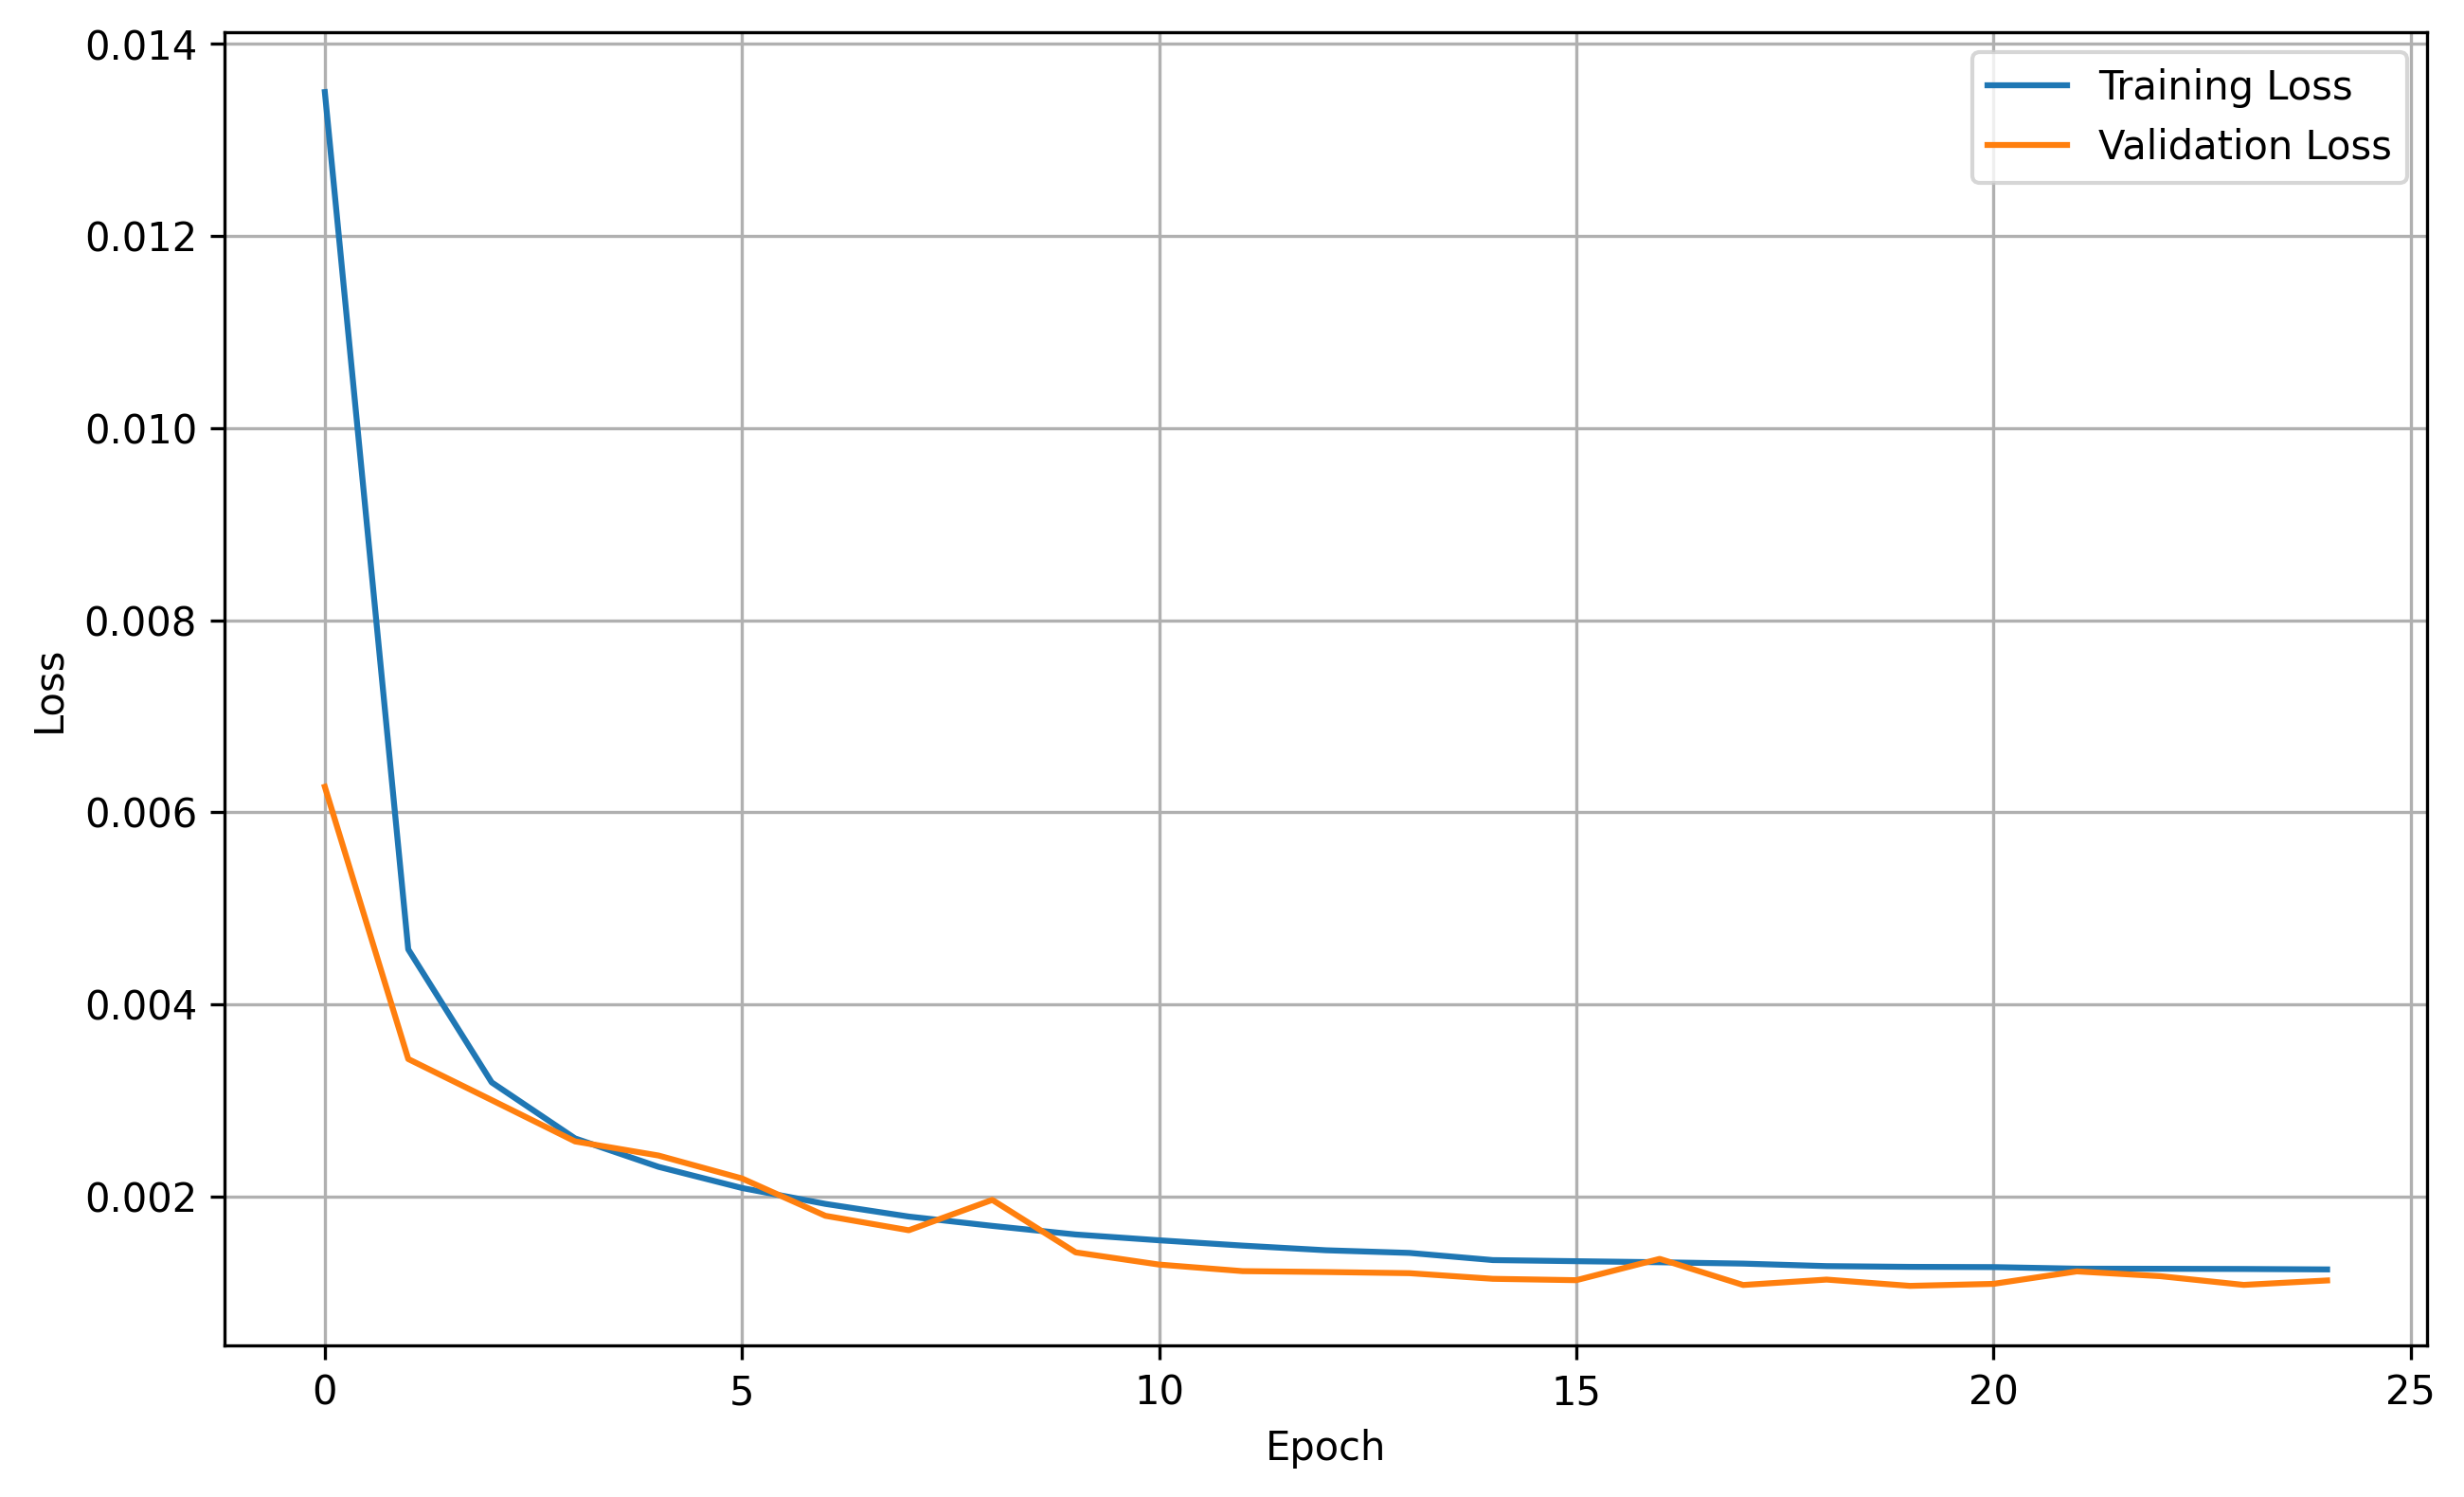
\includegraphics[width=10cm]{sections/figures/lstm_point_model_loss_during_training.png}
  \caption{LSTM 1-hour Model Loss During Training}
  \label{fig:lstm-point-model-loss-during-training}
\end{figure}

\begin{figure}[ht]
  \centering
  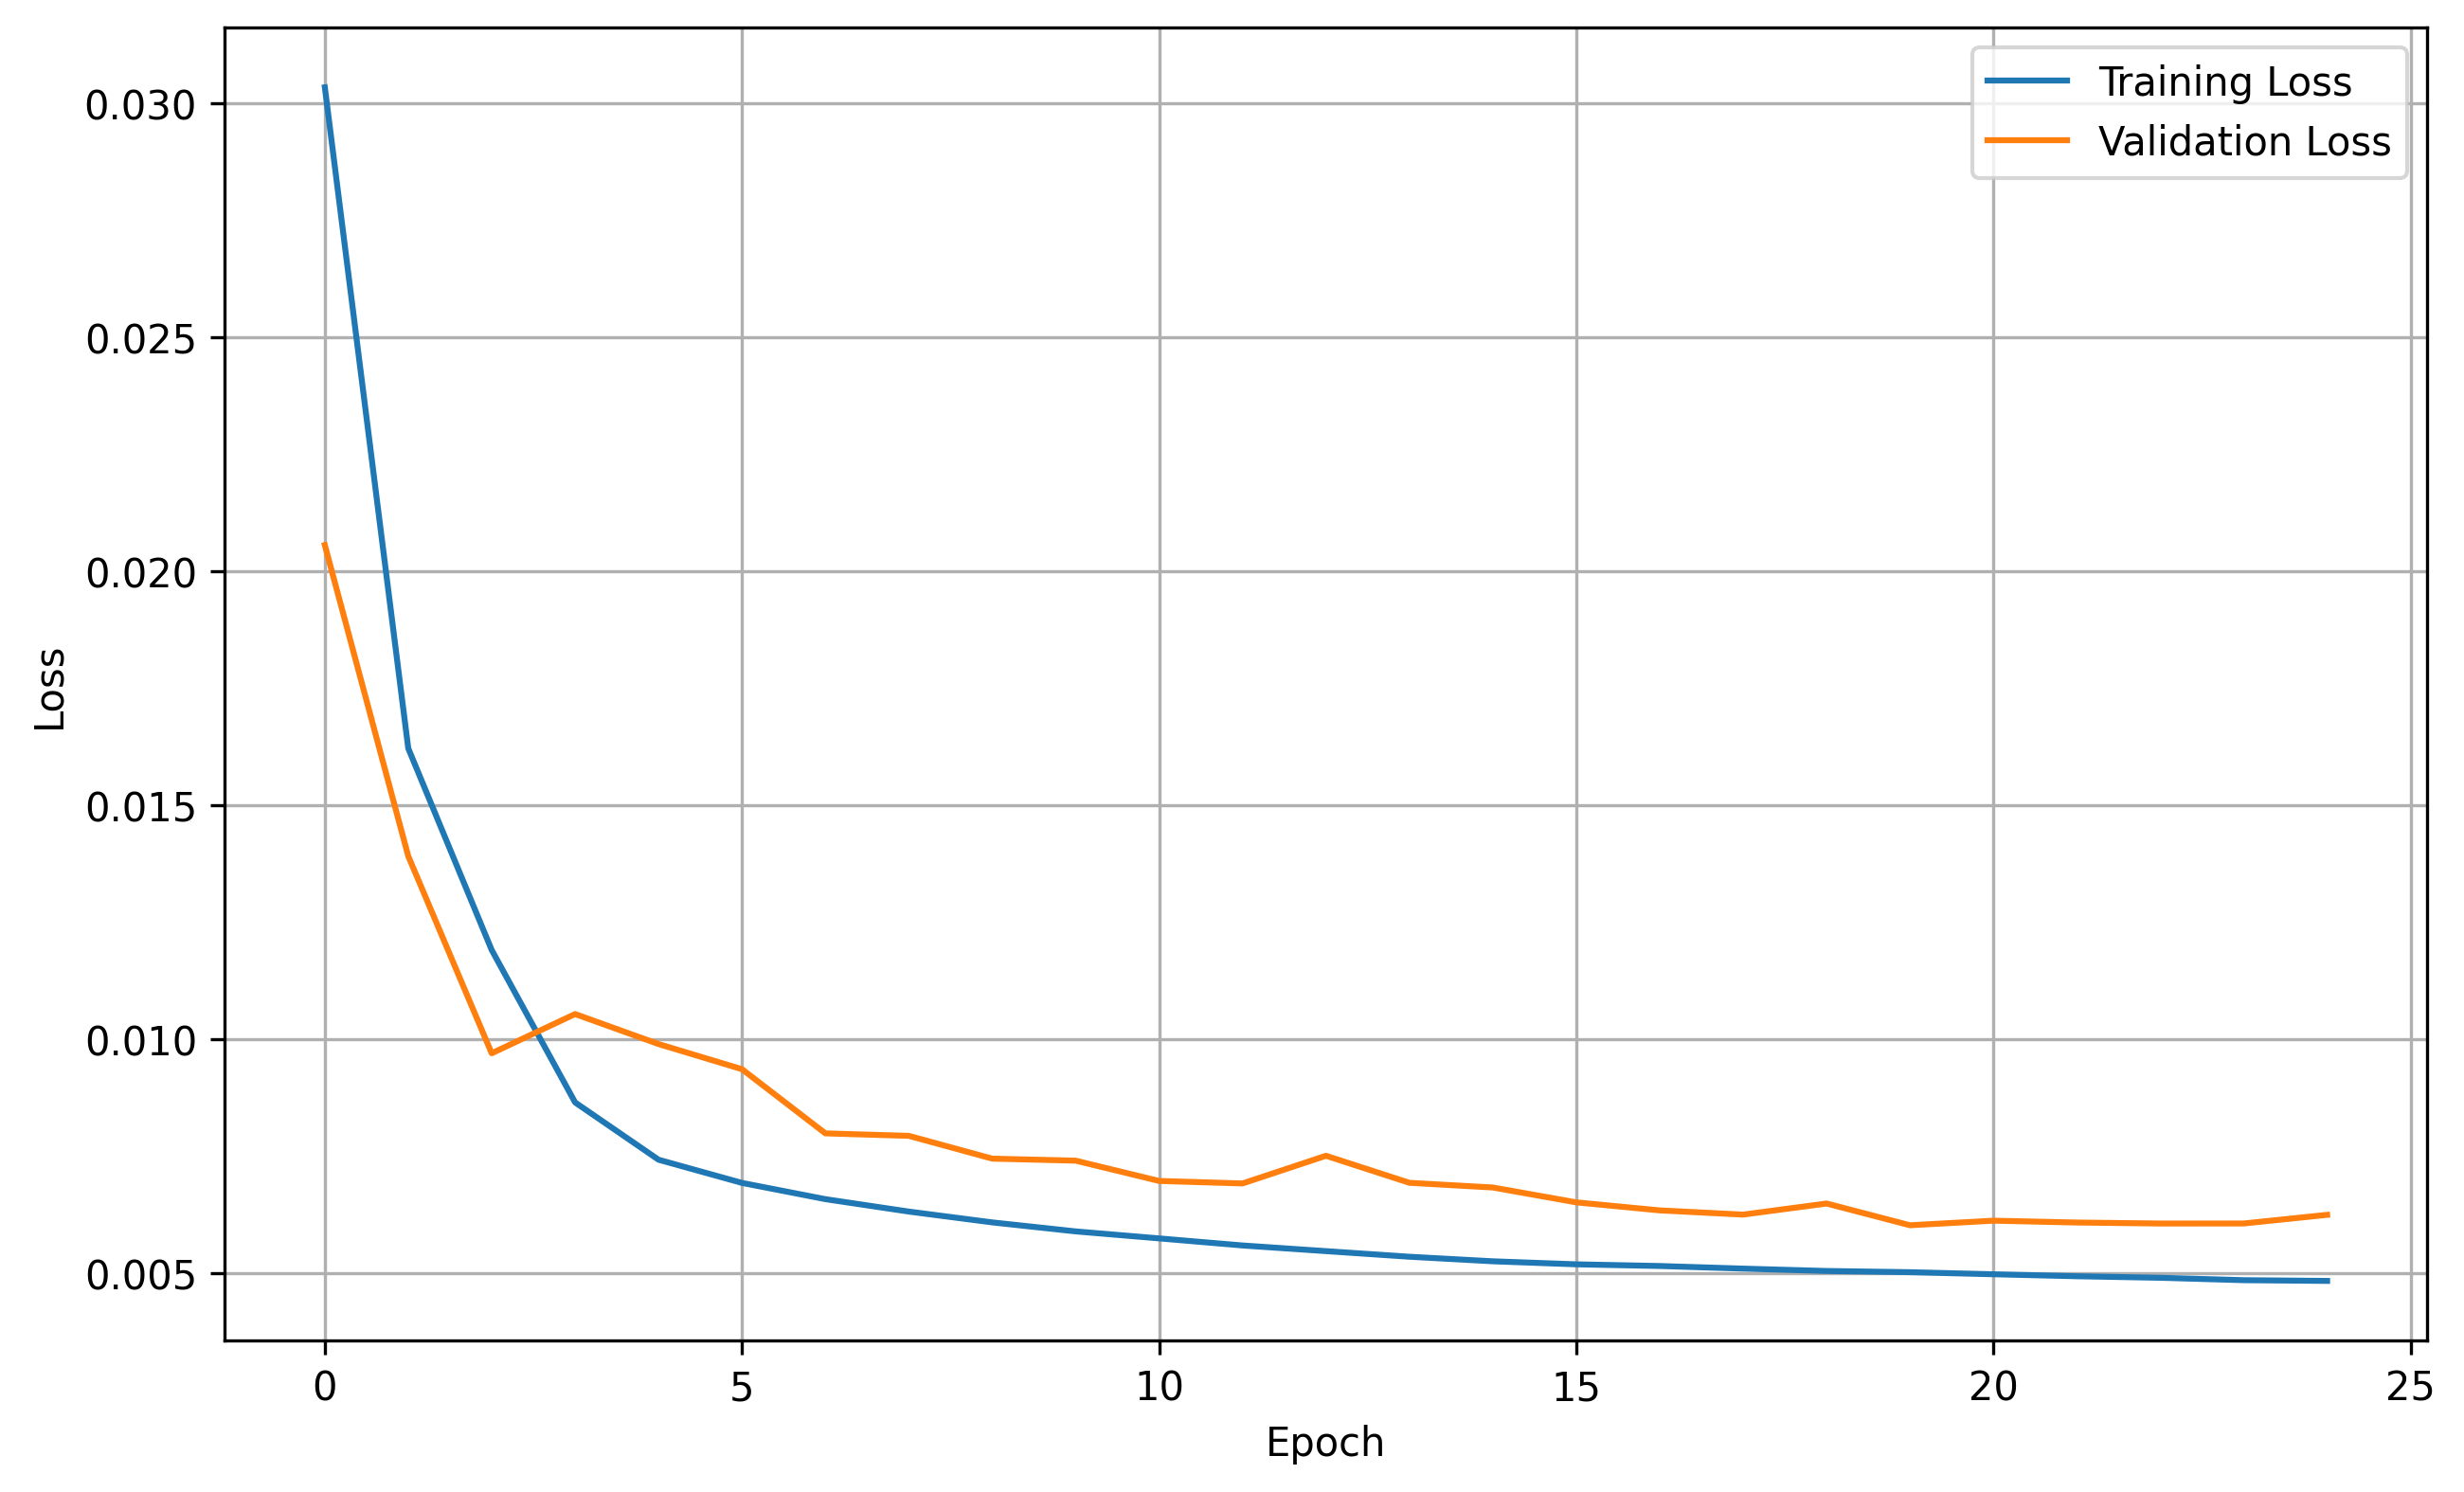
\includegraphics[width=10cm]{sections/figures/lstm_seq_model_loss_during_training.png}
  \caption{LSTM 24-hour Model Loss During Training}
  \label{fig:lstm-seq-model-loss-during-training}
\end{figure}

The training dynamics are illustrated in the loss curves for both architectures (\autoref{fig:lstm-point-model-loss-during-training} and \autoref{fig:lstm-seq-model-loss-during-training}), which exhibit the expected convergence patterns for well-configured LSTM models. Both the 1-hour and 24-hour models show rapid initial loss reduction during the first few epochs, followed by gradual convergence toward optimal performance levels. The training and validation losses track closely throughout the optimization process, with validation loss remaining slightly higher than training loss as expected, demonstrating effective generalization without significant overfitting. The absence of divergence between training and validation curves confirms that the models learned meaningful temporal patterns rather than memorizing training sequences, validating the robustness of the selected hyperparameter configurations for carbon emission forecasting in volatile wind power grids.

\subsection{LSTM Forecasting Results}

Following the hyperparameter optimization and training procedures outlined in the previous subsection, this section presents a comprehensive evaluation of LSTM forecasting performance across both prediction horizons. The analysis proceeds through residual diagnostics to assess model behavior and prediction quality, followed by performance comparisons against the established baseline models and statistical significance testing to validate the empirical improvements achieved by the LSTM architectures.

The residual analysis provides essential insights into model performance characteristics and potential systematic biases. For the 1-hour LSTM model, the residual distribution (\autoref{fig:lstm-point-test-residuals-frequency}) exhibits a approximately normal distribution centered near zero, indicating unbiased predictions with no systematic over- or under-prediction tendencies. The residual spread ranges primarily between -40 and +40 tonnes \cotwoe{}, with the majority of prediction errors concentrated within ±20 tonnes, demonstrating reasonable prediction accuracy for short-term forecasting applications. The temporal pattern of residuals (\autoref{fig:lstm-point-test-residuals-over-time}) reveals no obvious systematic trends or seasonal patterns in the errors, confirming that the model effectively captures the underlying temporal dependencies in carbon emission patterns without exhibiting time-dependent bias.

\begin{figure}[ht]
  \centering
  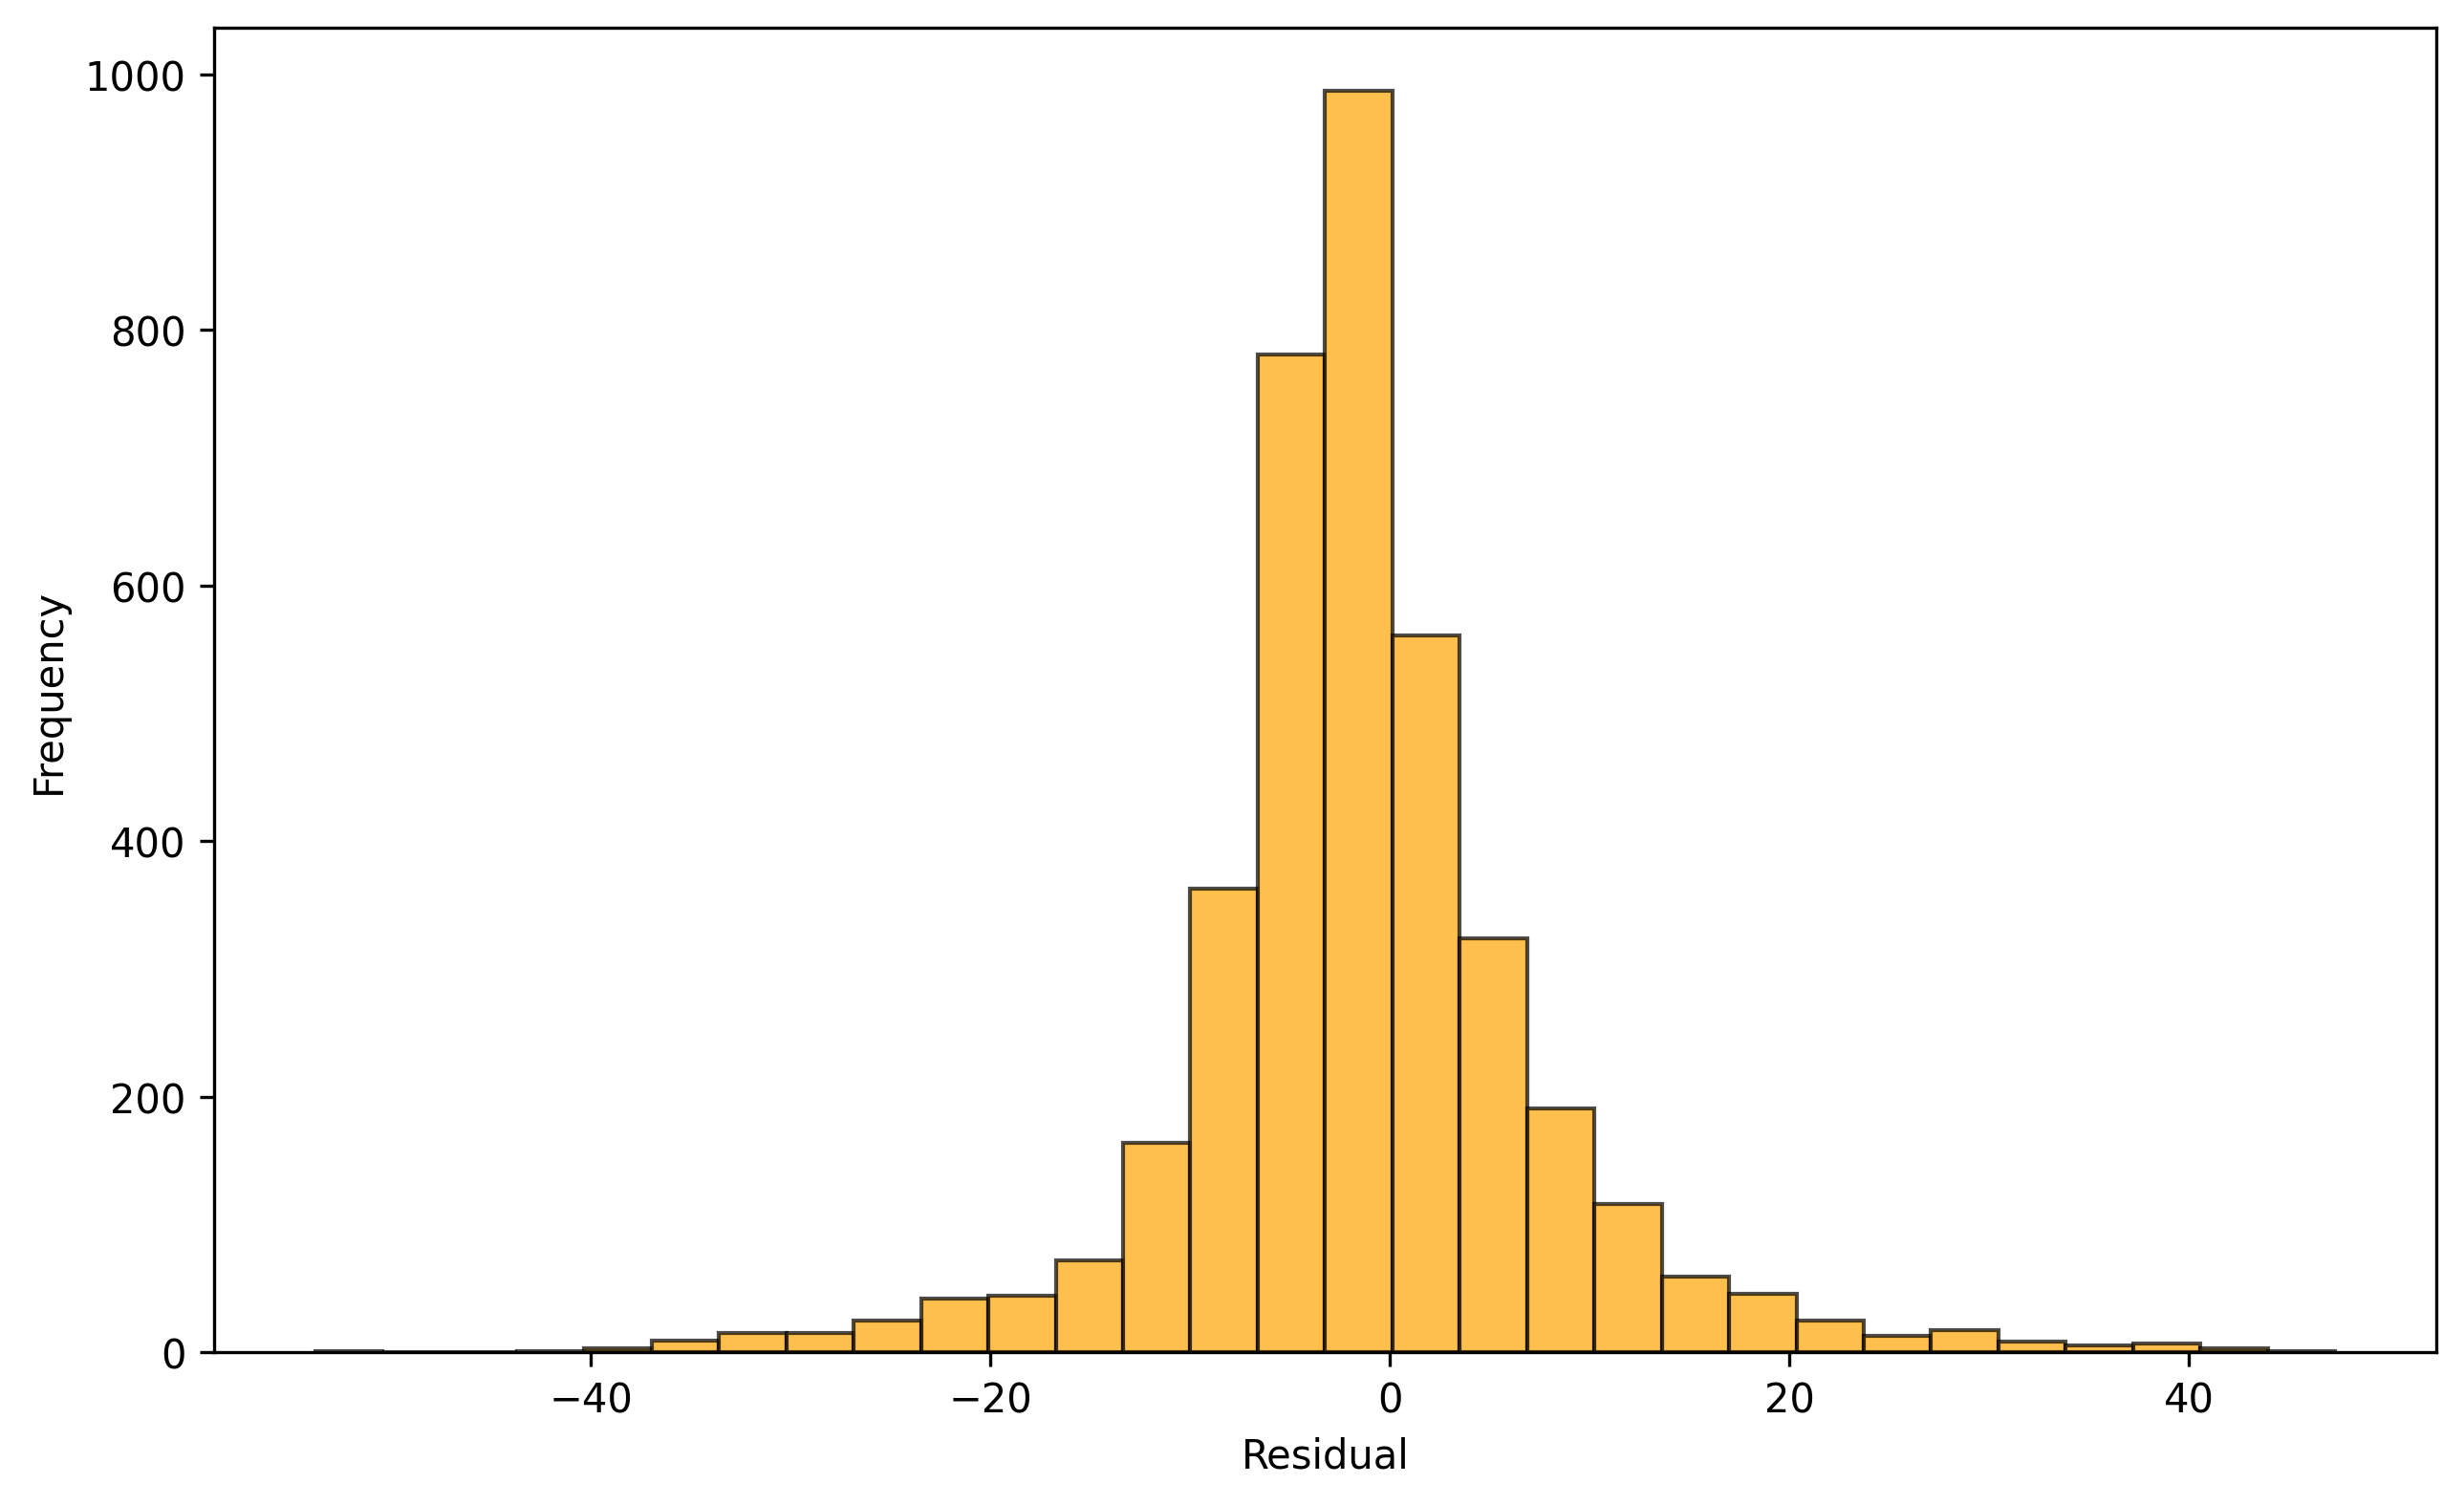
\includegraphics[width=10cm]{sections/figures/lstm_point_test_residuals_frequency.png}
  \caption{LSTM 1-hour Model Test Residuals Frequency}
  \label{fig:lstm-point-test-residuals-frequency}
\end{figure}

\begin{figure}[ht]
  \centering
  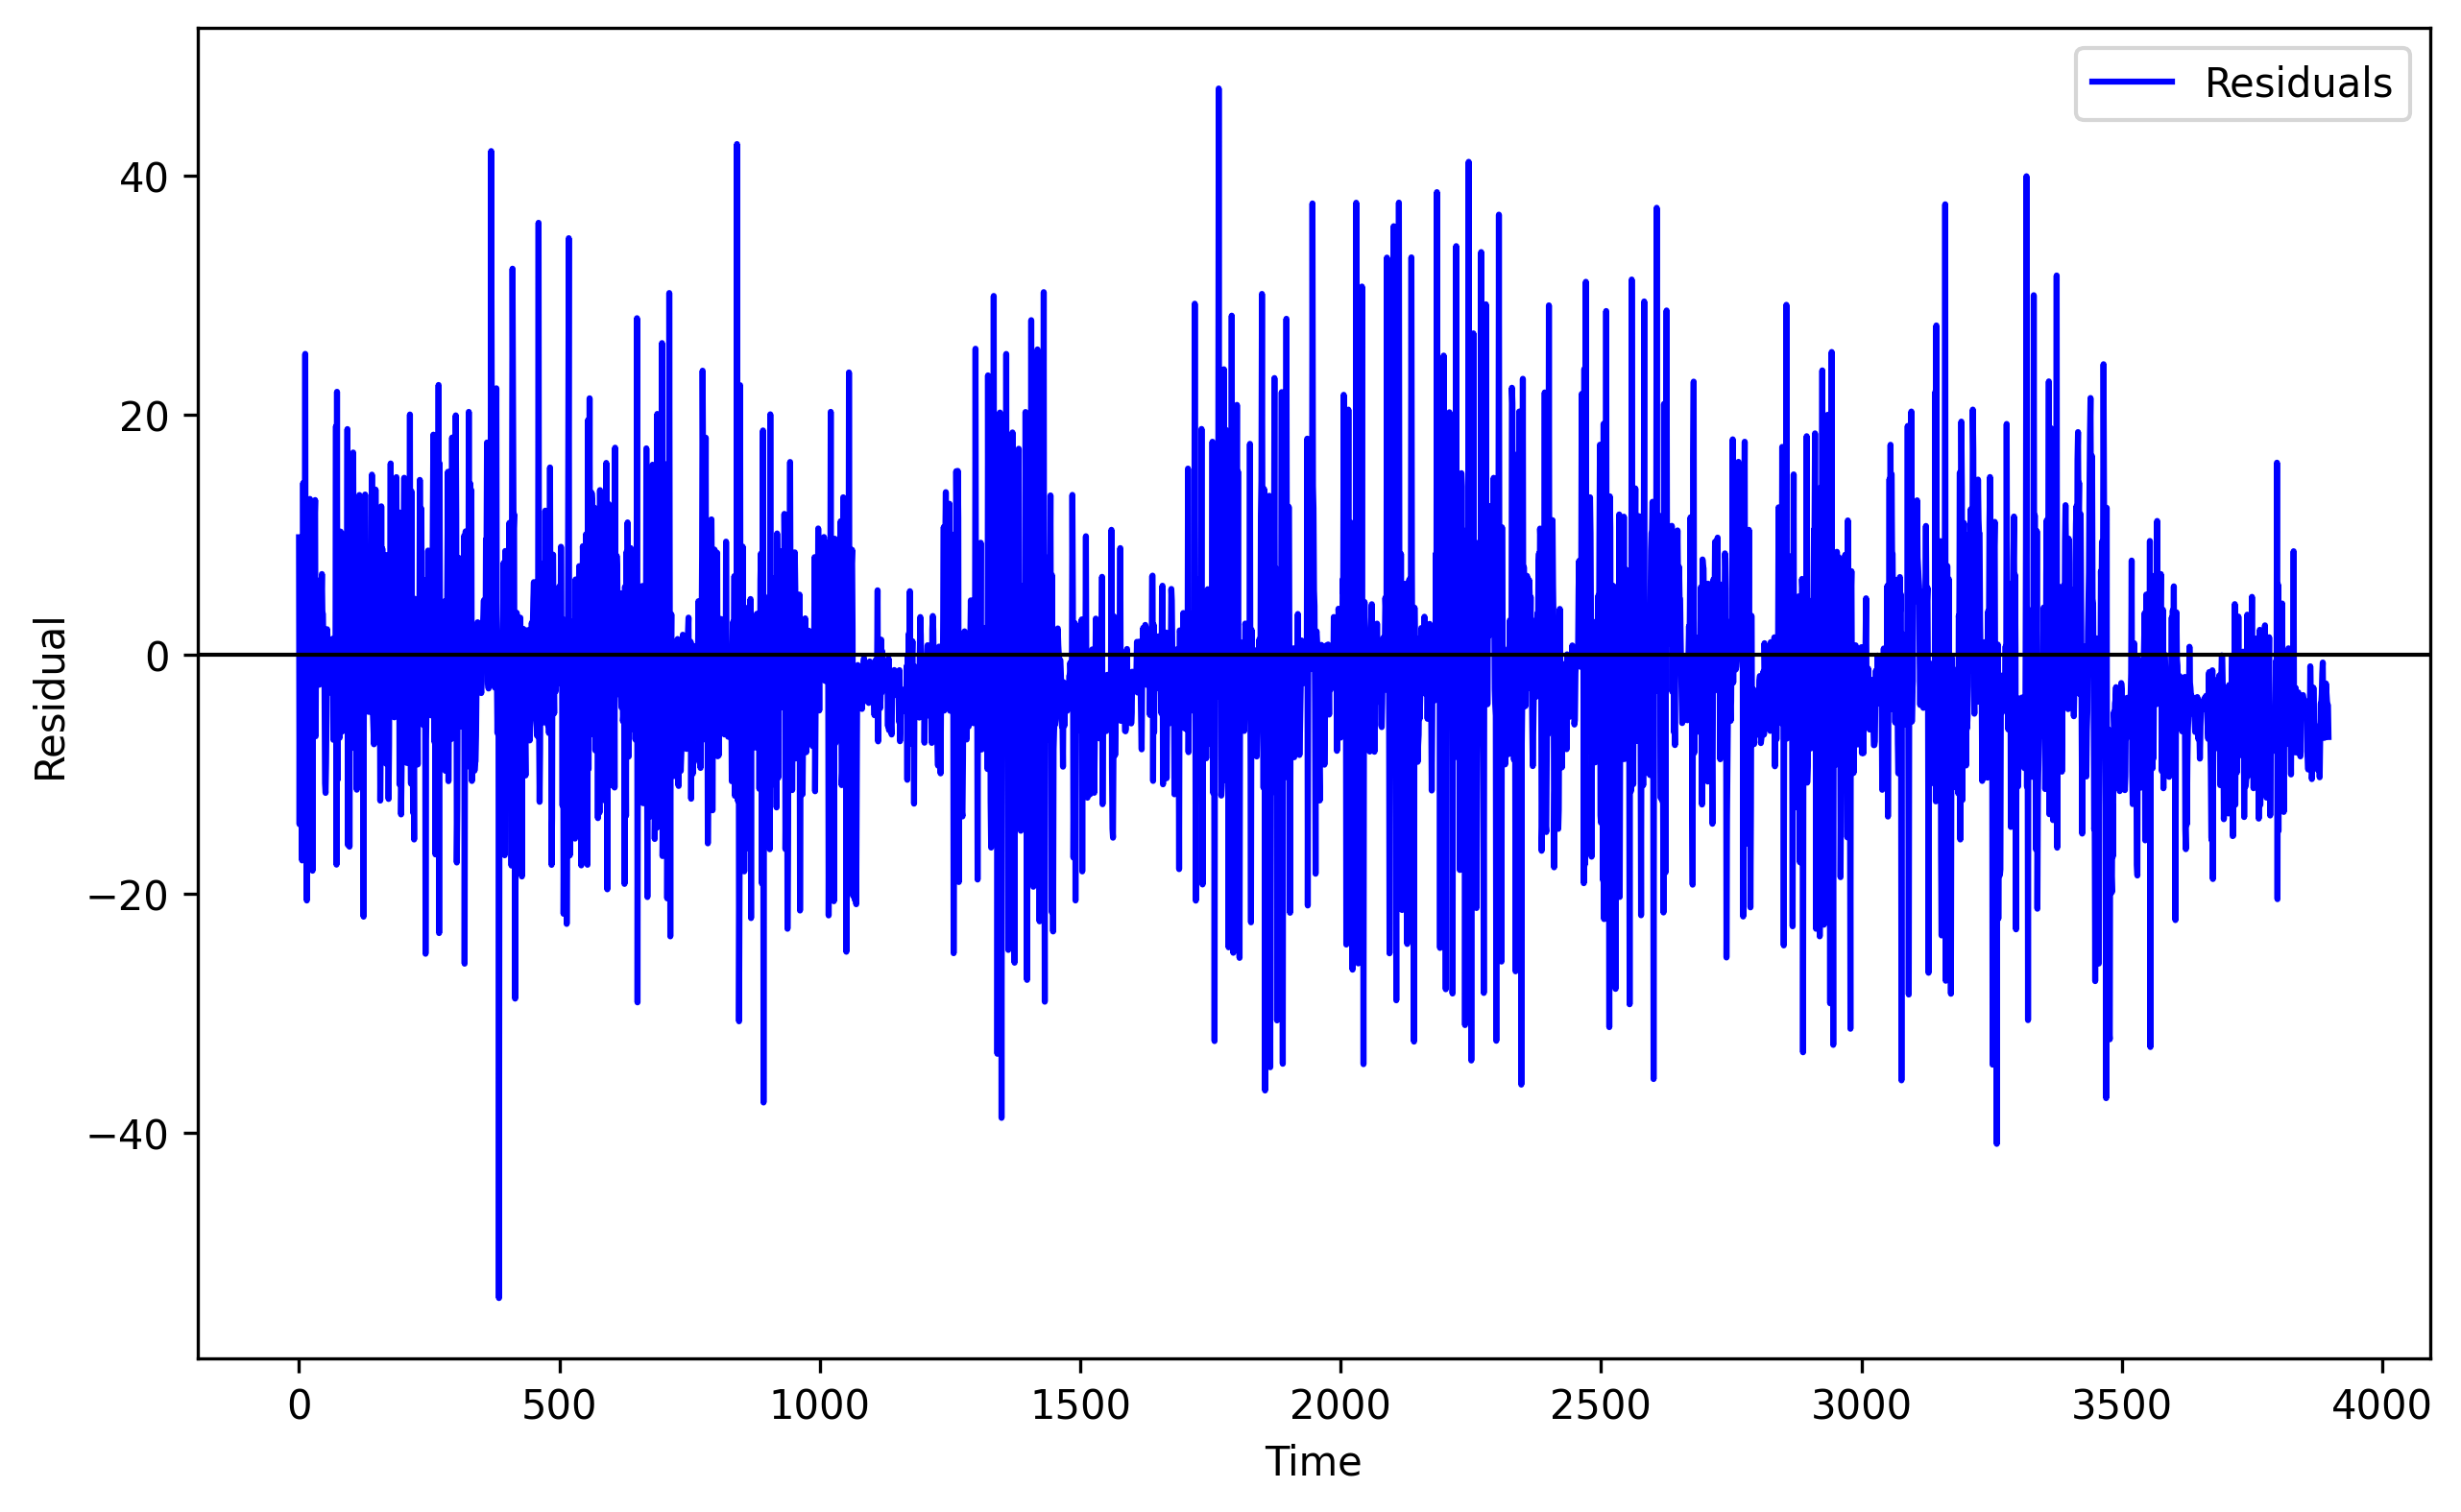
\includegraphics[width=10cm]{sections/figures/lstm_point_test_residuals_over_time.png}
  \caption{LSTM 1-hour Model Test Residuals Over Time}
  \label{fig:lstm-point-test-residuals-over-time}
\end{figure}

The 24-hour LSTM model demonstrates similar residual characteristics, though with appropriately larger error magnitudes reflecting the increased complexity of an extended forecasting horizon. The residual distribution (\autoref{fig:lstm-seq-test-residuals-frequency}) maintains a near-normal distribution centered at zero, with residuals primarily ranging between -75 and +75 tonnes \cotwoe{}. While the error spread is approximately double that of the 1-hour model, this increase is proportionally reasonable given the substantially longer prediction horizon and the cumulative uncertainty inherent in multi-step forecasting. The temporal residual pattern (\autoref{fig:lstm-seq-test-residuals-over-time}) similarly shows no systematic temporal bias, indicating effective learning of long-term dependencies across the 24-hour prediction sequences.

\begin{figure}[ht]
  \centering
  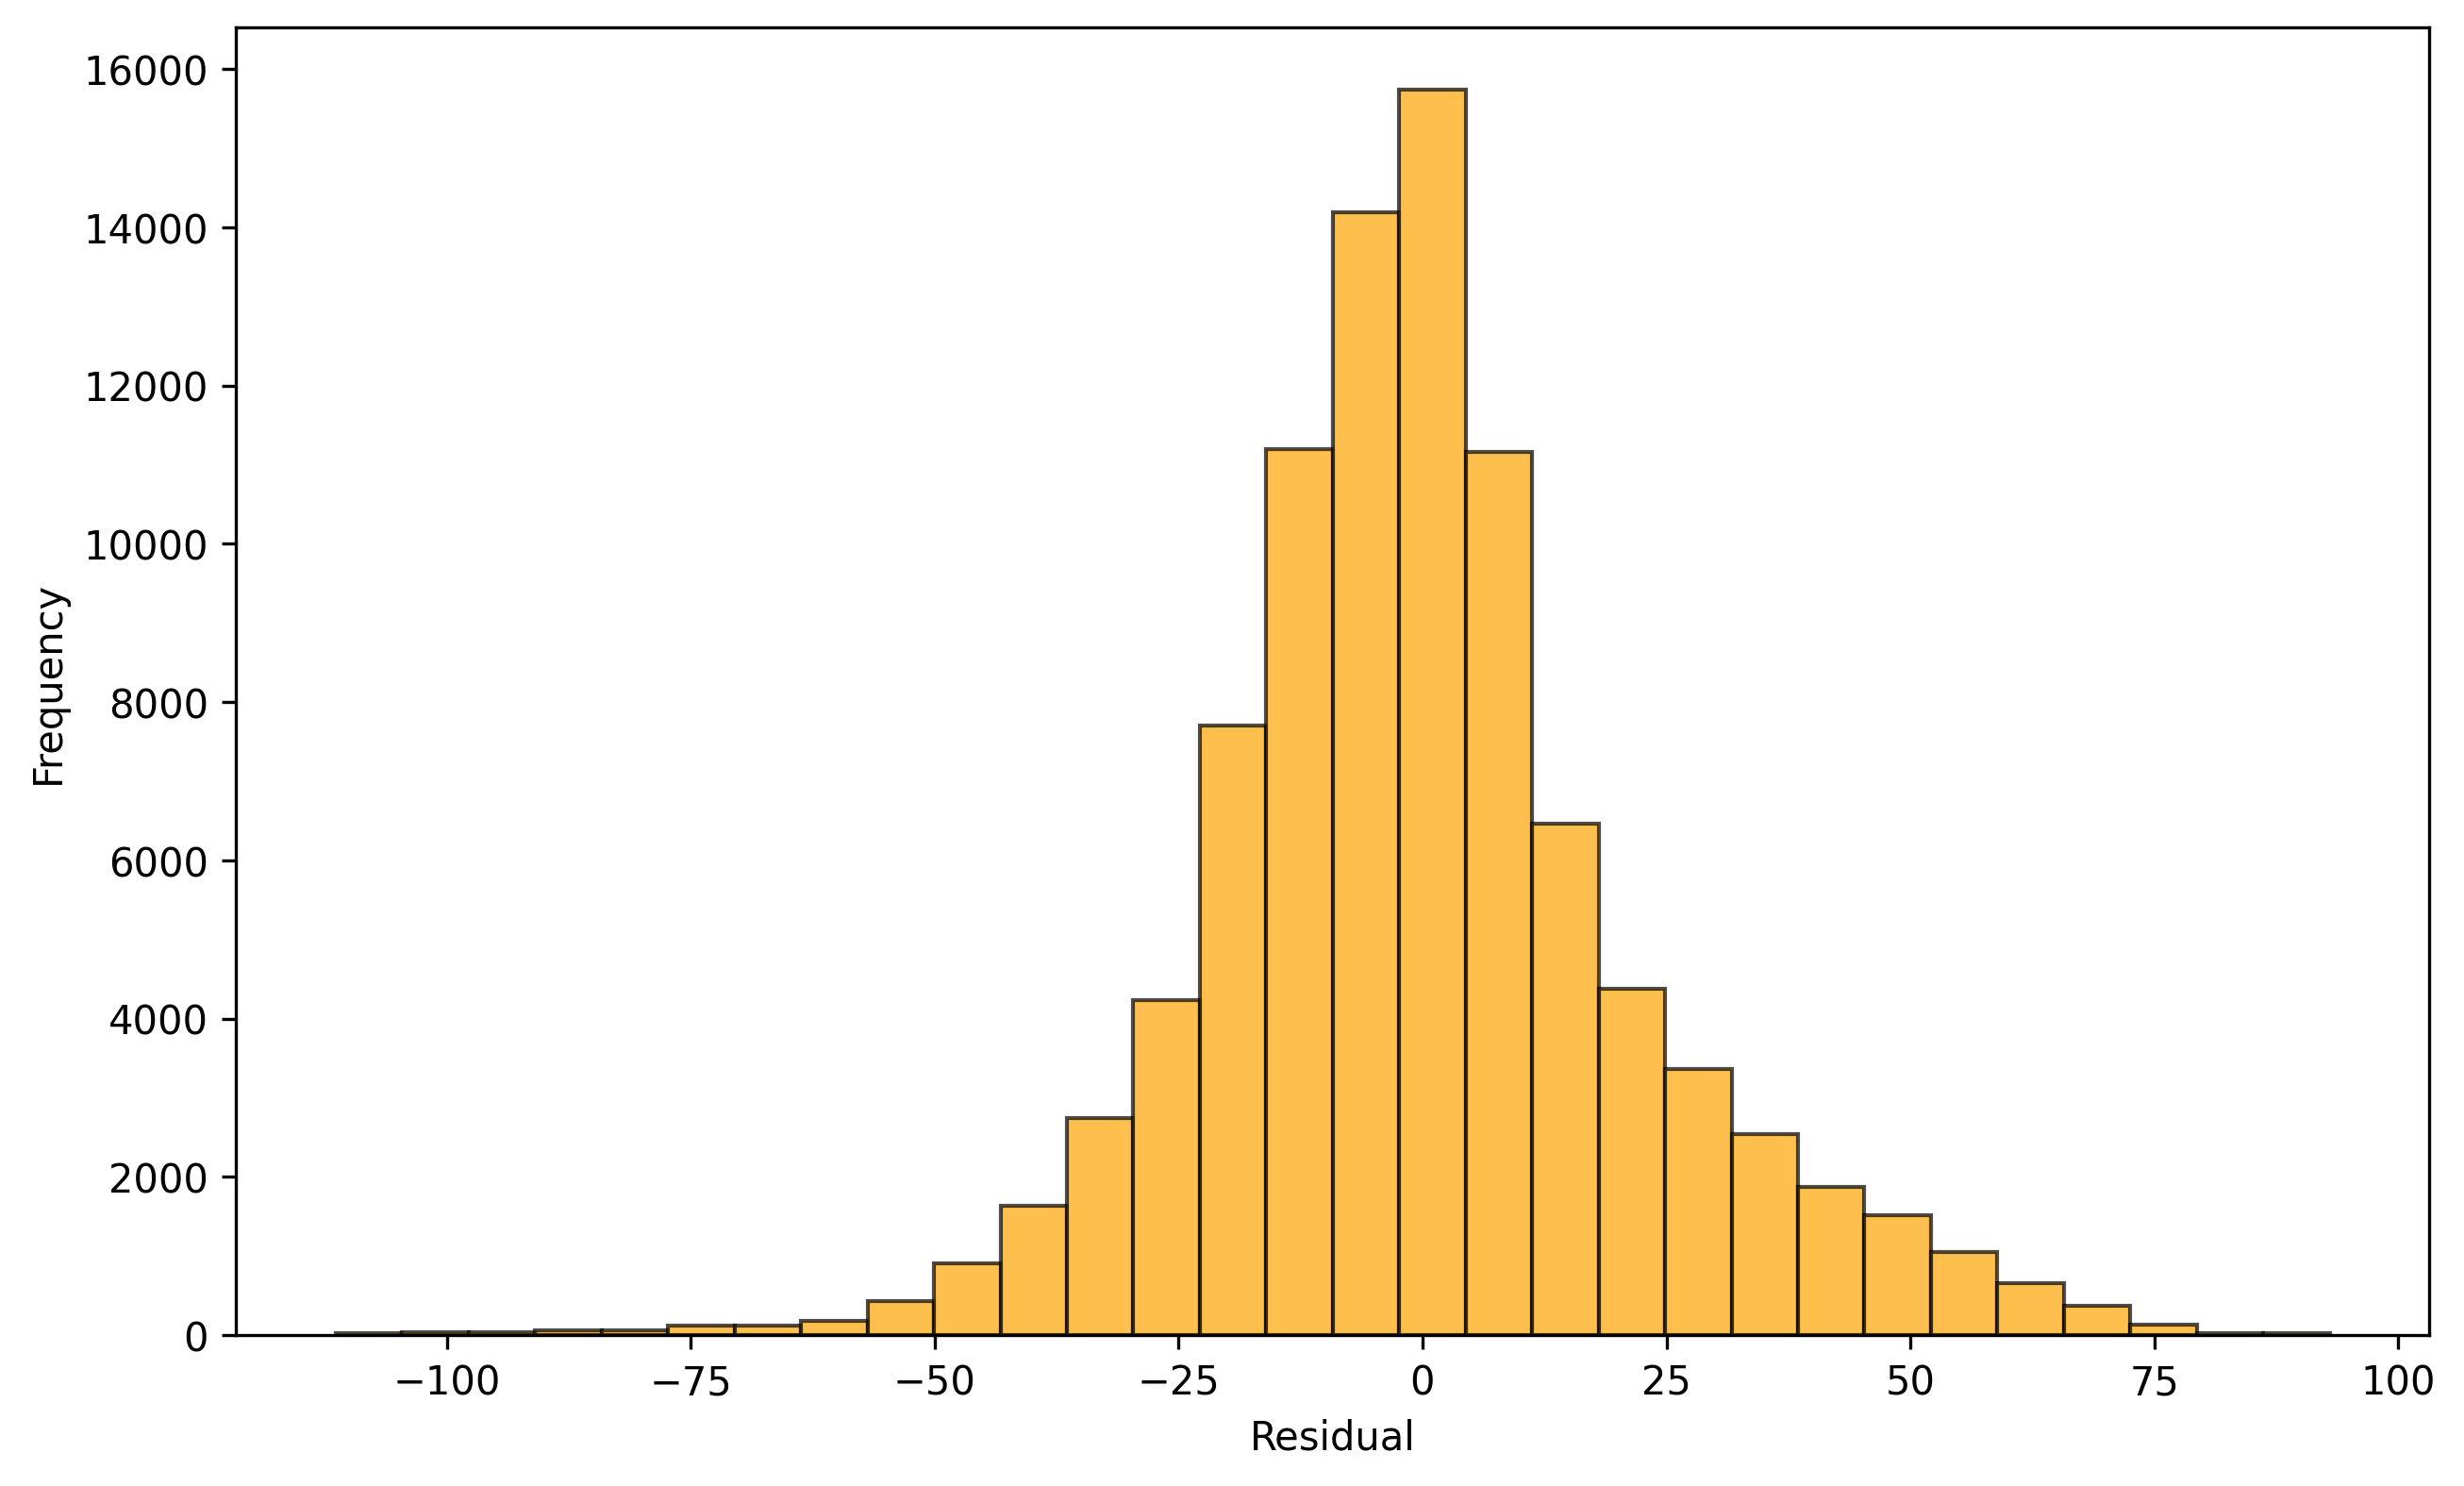
\includegraphics[width=10cm]{sections/figures/lstm_seq_test_residuals_frequency.png}
  \caption{LSTM 24-hour Model Test Residuals Frequency}
  \label{fig:lstm-seq-test-residuals-frequency}
\end{figure}

\begin{figure}[ht]
  \centering
  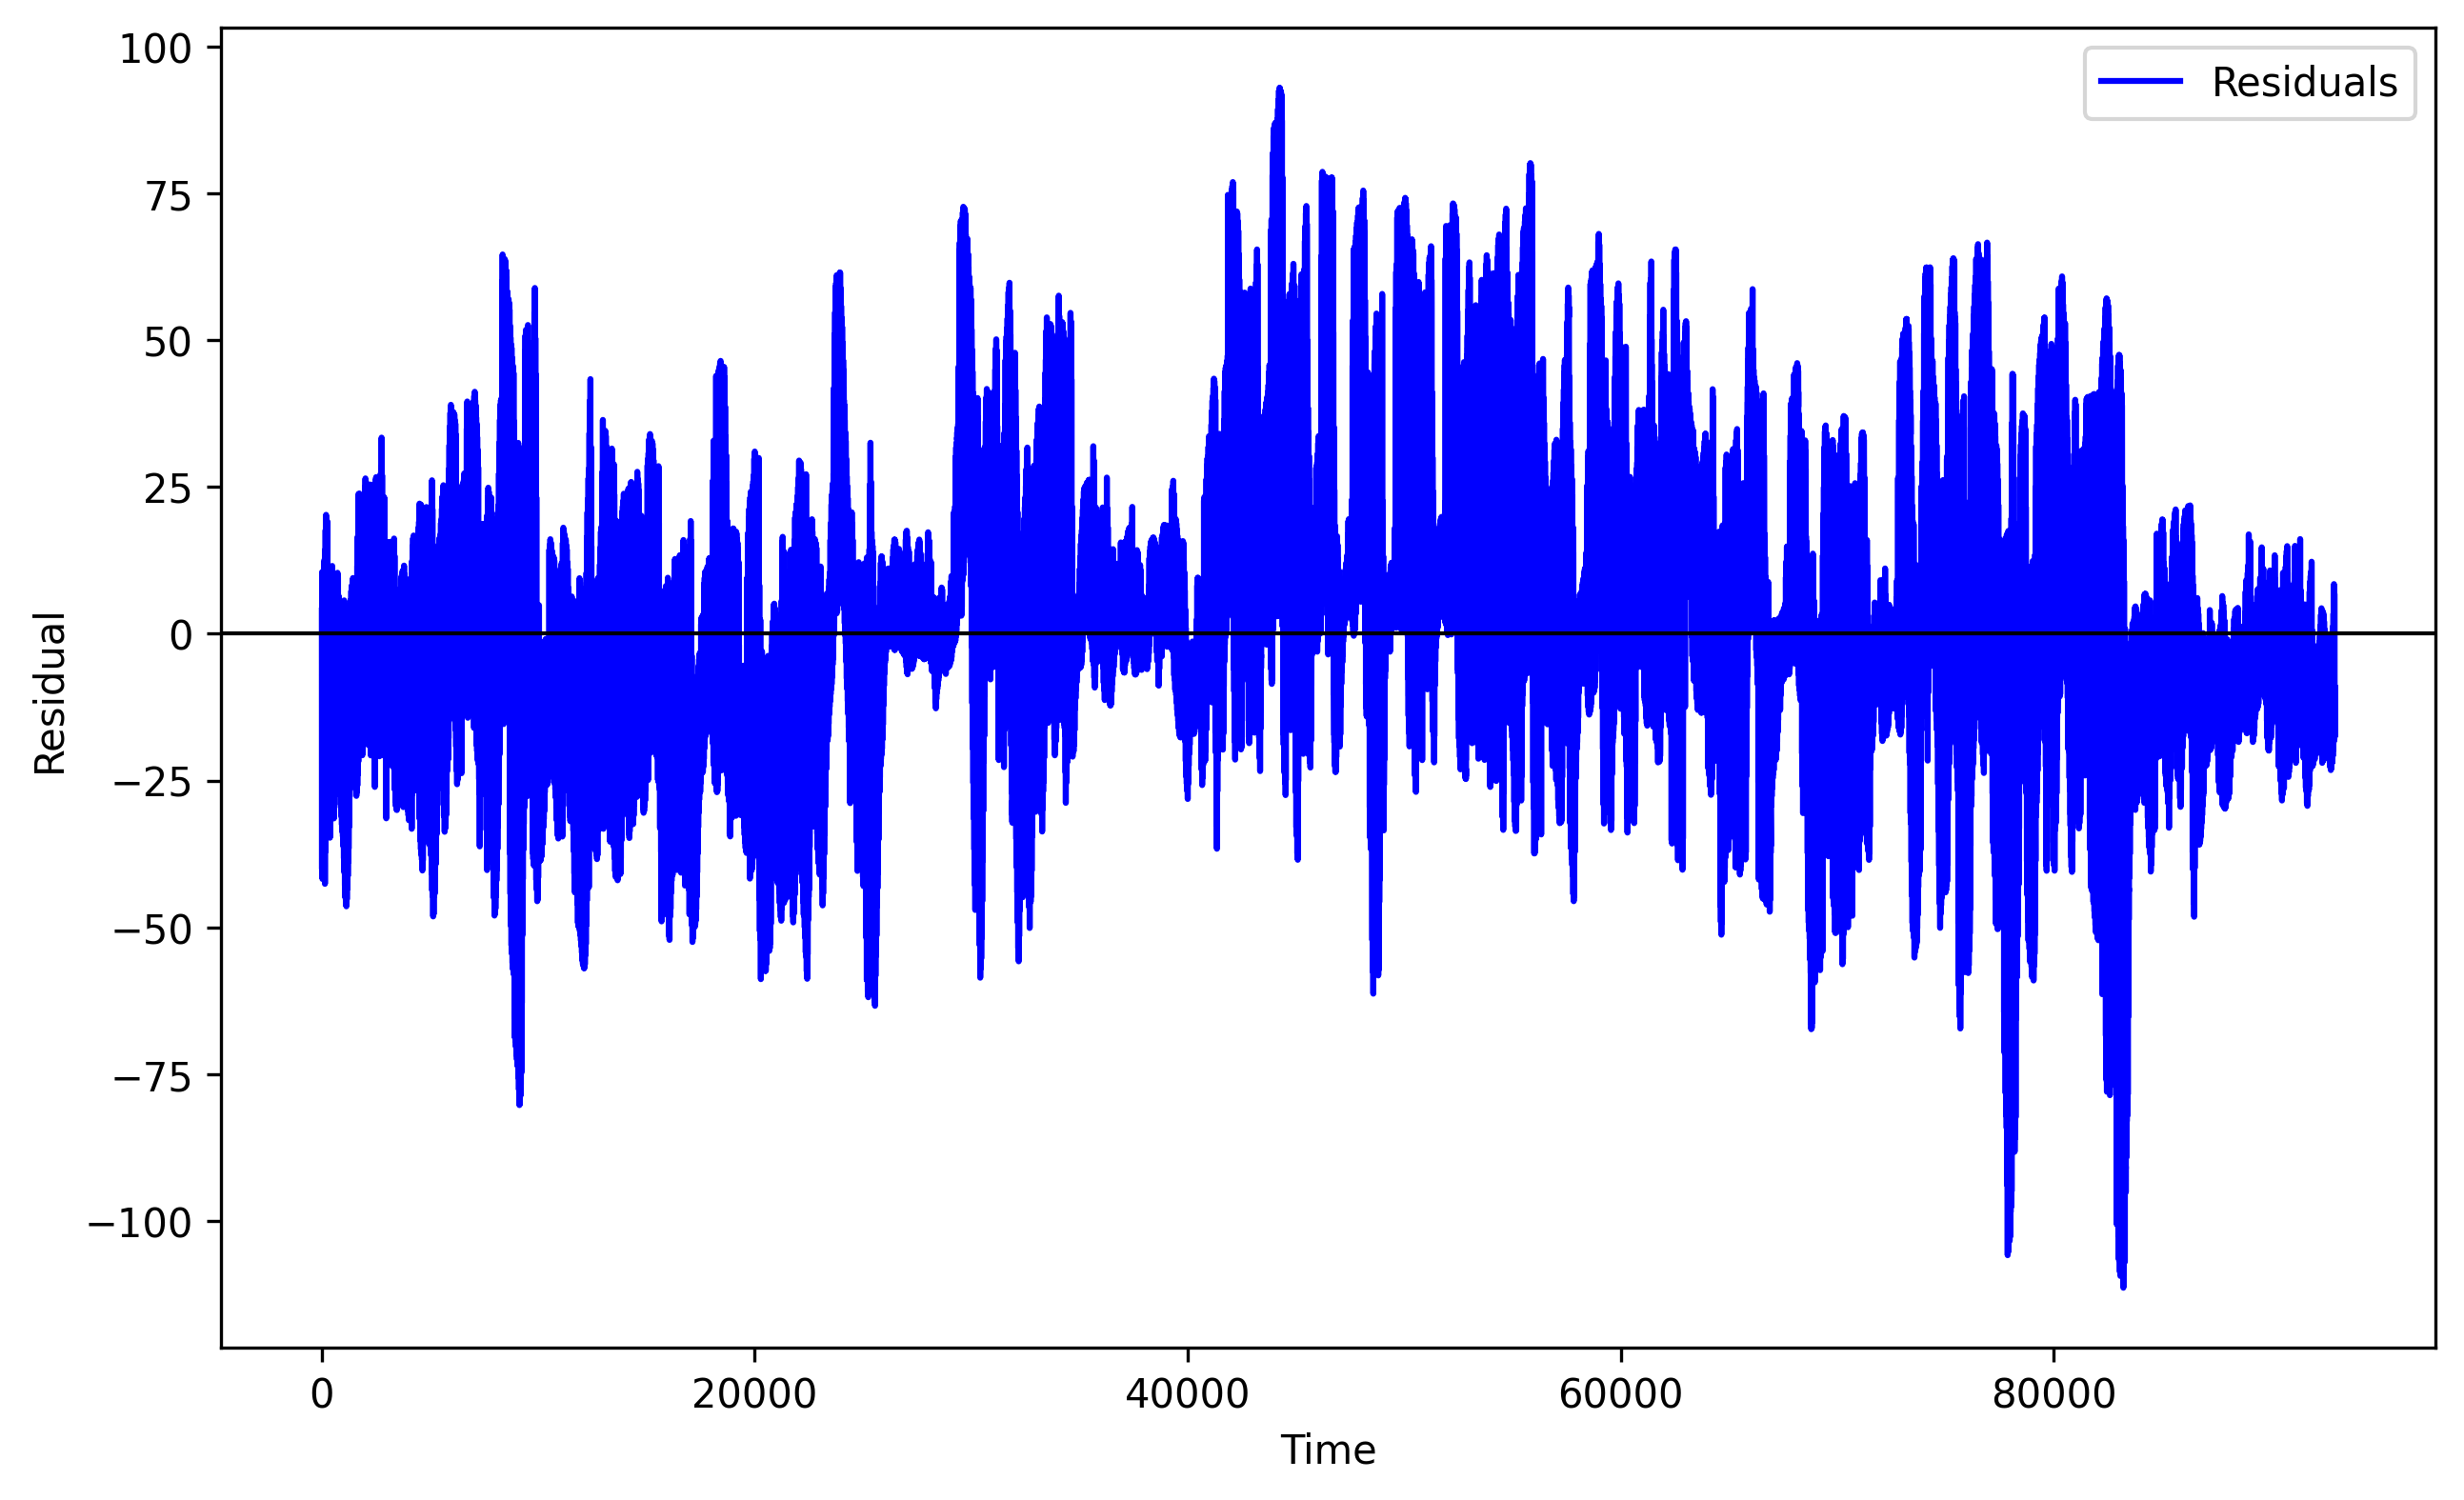
\includegraphics[width=10cm]{sections/figures/lstm_seq_test_residuals_over_time.png}
  \caption{LSTM 24-hour Model Test Residuals Over Time}
  \label{fig:lstm-seq-test-residuals-over-time}
\end{figure}

Representative prediction examples (shown in \autorefapdx{apdx:lstms-predictions-vs-actuals}) illustrate the practical forecasting capabilities of both LSTM architectures. The 1-hour model predictions (\autoref{fig:lstm-point-test-pred-vs-acts}) demonstrate close tracking of actual carbon emission patterns across various operational scenarios, capturing both gradual trends and more volatile fluctuations characteristic of wind-dominated grids. The model effectively follows the directional changes in emissions while maintaining reasonable accuracy during periods of rapid variation. For the 24-hour model (\autoref{fig:lstm-seq-test-pred-vs-acts}), the sequence predictions show strong performance in capturing overall emission trends and patterns across the full prediction horizon. While some divergence between predicted and actual values becomes apparent in the later hours of certain sequences, the model generally maintains directional accuracy and captures the fundamental emission patterns driven by renewable generation variability and demand cycles.

Comparative performance evaluation reveals substantial improvements over baseline approaches across both forecasting horizons. For 1-hour-ahead prediction, the LSTM model achieved a test RMSE of 9.01 and MAE of 6.28, representing a 14.5\% decrease in RMSE compared with the naive persistence baseline (RMSE = 10.54, MAE = 6.13), albeit with a 2.4\% increase in MAE. Relative to the ARIMA model (RMSE = 9.43, MAE = 5.99), the LSTM delivered a 4.5\% decrease in RMSE while showing a 4.8\% increase in MAE. The 24-hour forecasting results are even more pronounced: the LSTM obtained an RMSE of 22.20 and MAE of 16.32, corresponding to decreases of 25.4\% in RMSE and 19.7\% in MAE over naive persistence (RMSE = 29.75, MAE = 20.33). Compared with the ARIMA benchmark (RMSE = 25.03, MAE = 18.21), the LSTM achieves decreases of 11.3\% in RMSE and 10.4\% in MAE. For a comprehensive overview of all model error metrics across train, test, and validation splits see \autoref{tab:overview-maes-across-models} and \autoref{tab:overview-rmse-across-models} in \autorefapdx{apdx:comprehensive-model-error-metrics}.

Statistical significance testing through two-sided Diebold-Mariano tests confirms that these performance improvements represent meaningful advances rather than random variation. For the 1-hour forecasting task, the LSTM significantly outperformed both the naive baseline (DM statistic = -10.05, \(p < 0.0001\)) and the ARIMA model (DM statistic = -3.67, \(p = 0.0002\)), enabling rejection of the null hypothesis of equal predictive accuracy. The 24-hour results show even stronger statistical evidence, with the LSTM demonstrating highly significant improvements over naive persistence (DM statistic = -19.12, \(p < 0.0001\)) and ARIMA (DM statistic = -9.65, \(p < 0.0001\)). These results provide robust statistical validation that the LSTM architectures deliver substantially improved carbon emission forecasting accuracy for volatile wind power grids, justifying the increased computational complexity through measurable and statistically significant performance gains across both operational forecasting horizons.

\subsection{Feature Importance Analysis}

Permutation importance analysis was conducted on the 24-hour LSTM model to empirically validate the relevance of selected explanatory variables and feature engineering choices. The analysis systematically evaluated all 43 features in the final dataset, measuring the degradation in model performance when each feature's values were randomly shuffled while maintaining all other features unchanged. Each permutation was repeated 10 times to ensure robust importance estimates, with scores calculated as the difference between baseline validation RMSE and post-permutation RMSE.

The results reveal a clear hierarchical structure in feature contributions. The top 10 contributions are shown in \autoref{fig:lstm-seq-feature-importance} and the full results can be viewed in \autorefapdx{apdx:full-feature-importance-analysis-results}. Historical carbon emissions dominated the importance rankings with a score of 22.58 tonnes \cotwoe{}, substantially exceeding all other features and confirming the strong autocorrelation inherent in carbon emission time series. Among exogenous variables, future solar photovoltaic production emerged as the most influential predictor with an importance score of 4.94, followed by future temperature forecasts (3.67) and future consumption (2.19). These findings validate the theoretical merit-order principles underlying variable selection, demonstrating that renewable generation forecasts and demand indicators directly contribute to predictive performance.

\begin{figure}[ht]
  \centering
  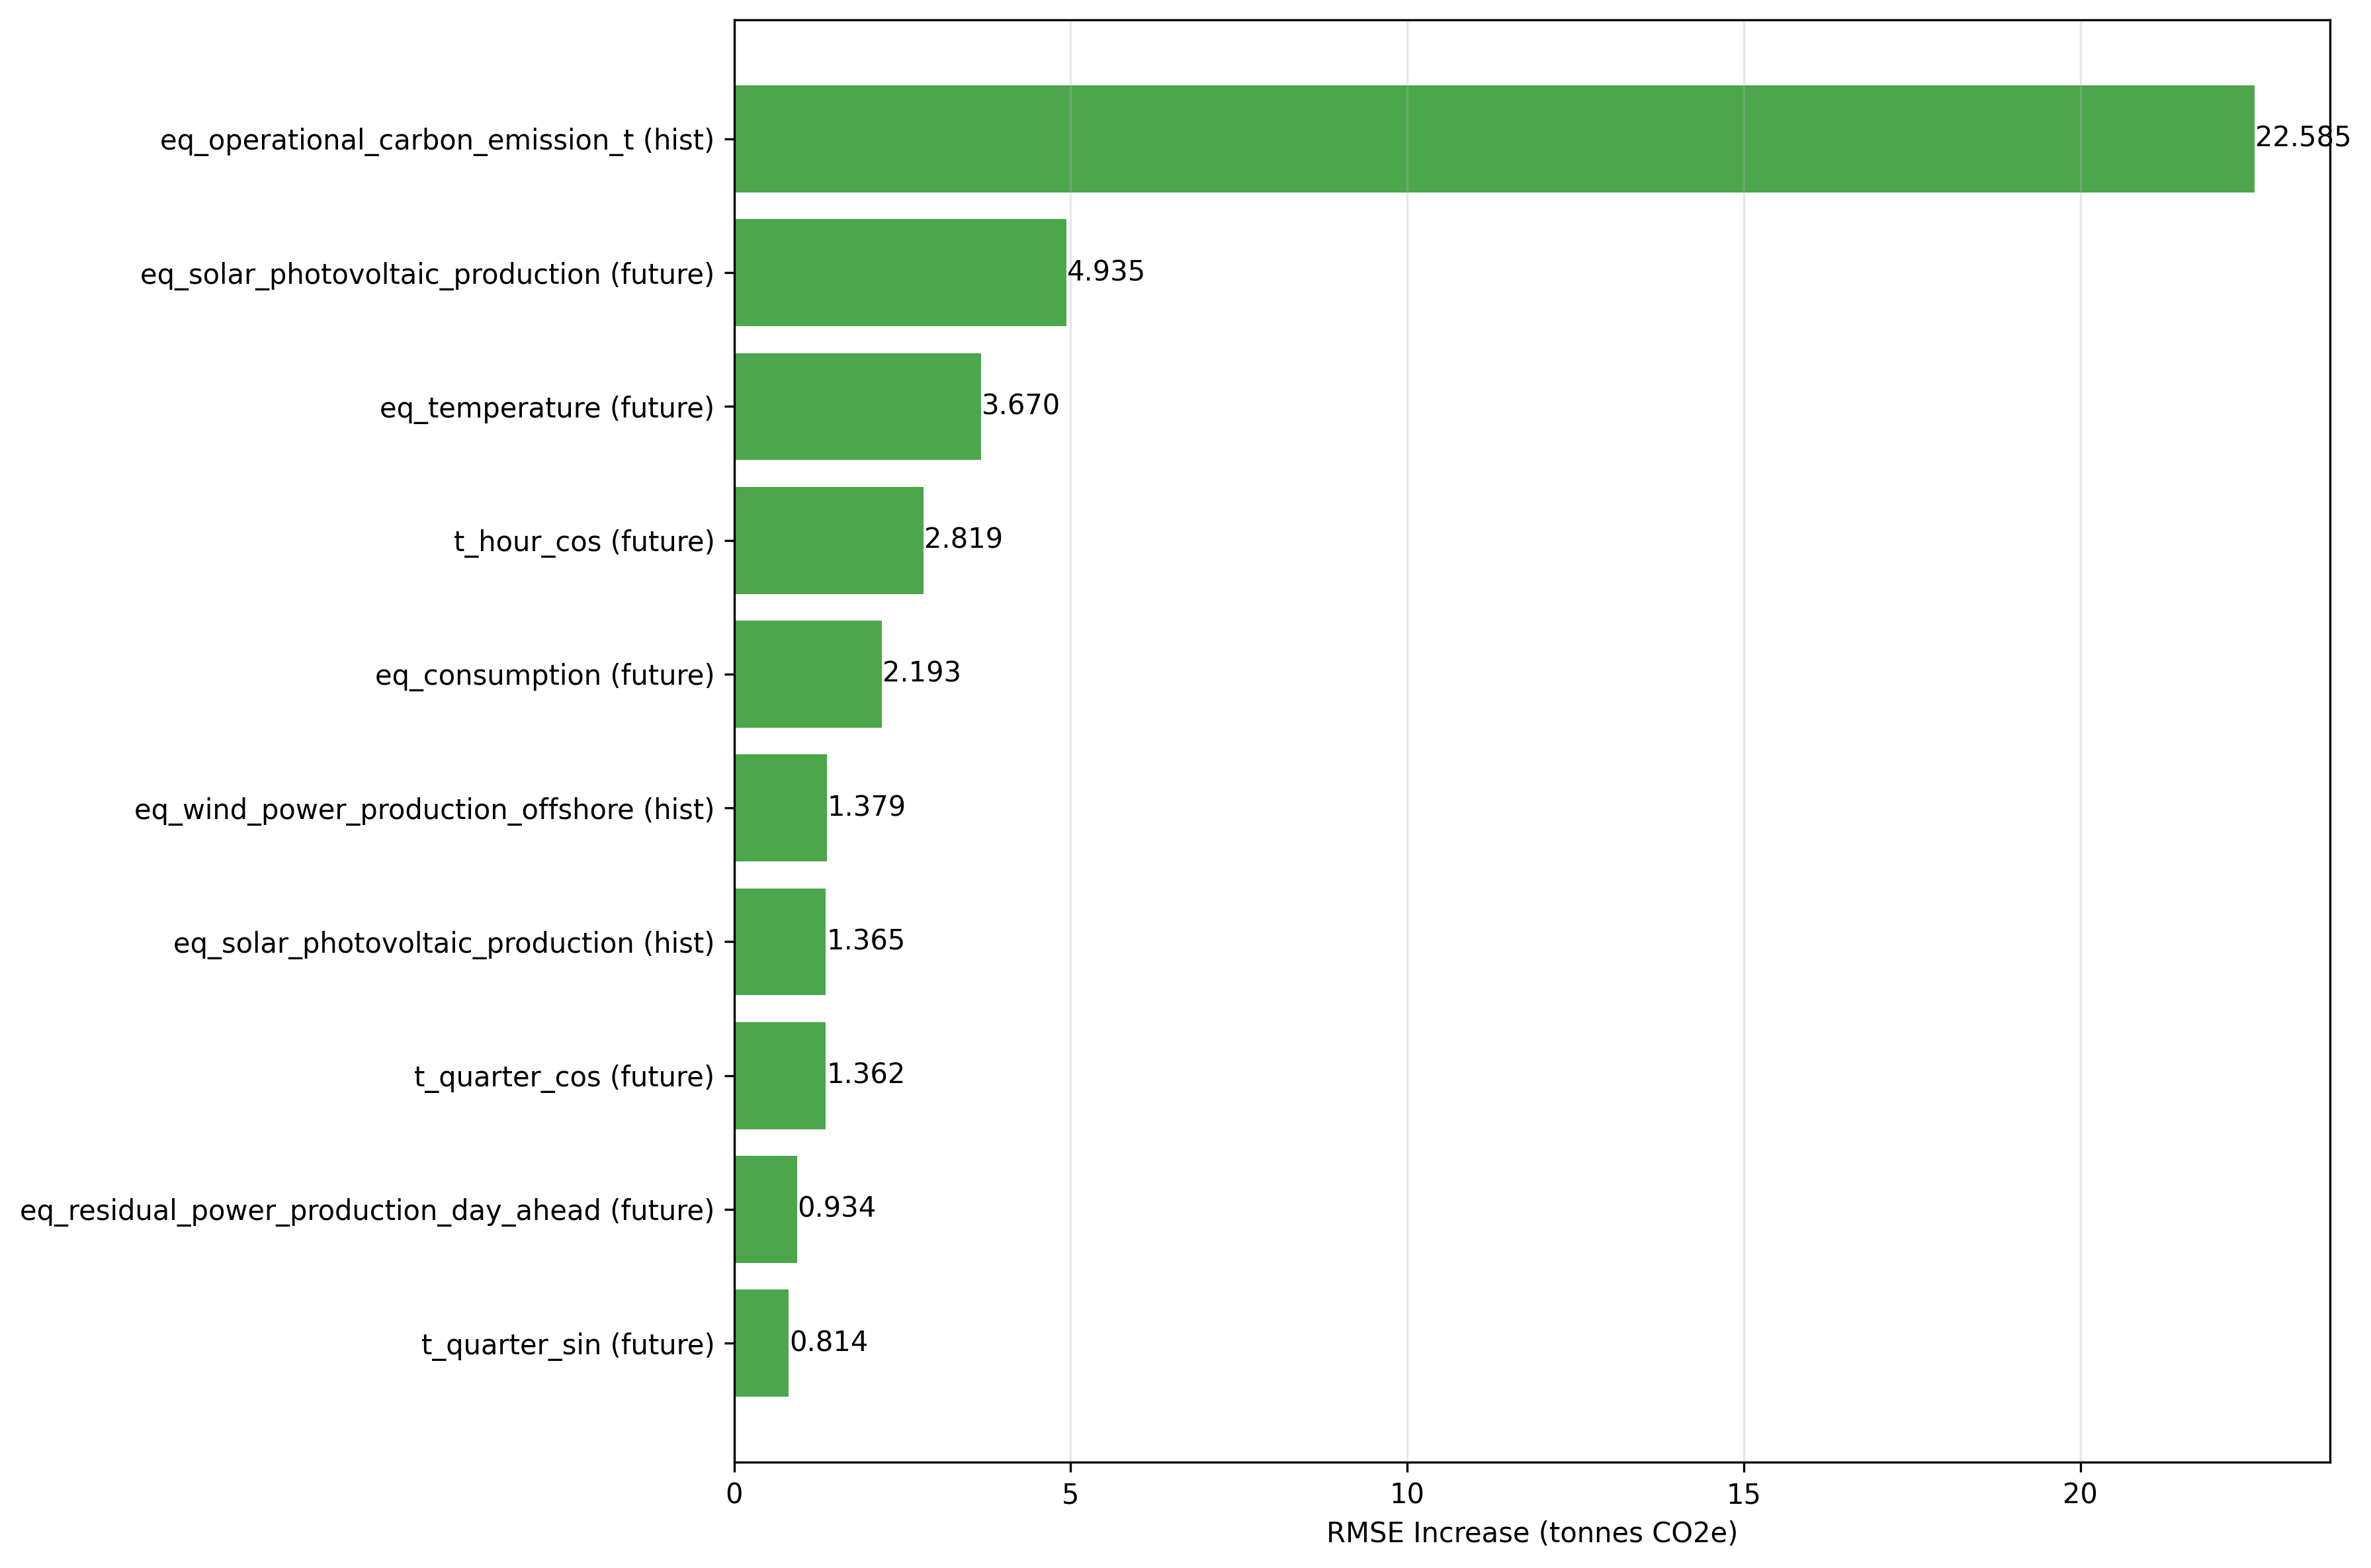
\includegraphics[width=16cm]{sections/figures/lstm_seq_feature_importance.png}
  \caption{LSTM 24-hour Model Feature Importance}
  \label{fig:lstm-seq-feature-importance}
\end{figure}

The analysis confirms the value of both supply-side and demand-side variables, with future renewable production features (solar photovoltaic, wind offshore, wind onshore) collectively contributing significant predictive power. Market-related variables including consumption, temperature, and residual production forecasts showed meaningful but moderate importance scores ranging from 0.93 to 2.19. Temporal features demonstrated mixed contributions, with future hourly cosine (2.82) and quarterly cosine (1.36) patterns showing notable importance, while several historical temporal features exhibited negative importance scores, suggesting potential noise contribution rather than predictive value.

The predominance of future exogenous variables over their historical counterparts validates the encoder-decoder architecture's design for incorporating day-ahead forecasts. The strong performance of renewable production variables confirms their theoretical importance in merit-order dispatch dynamics, while the significance of temperature and consumption forecasts demonstrates the model's ability to leverage demand-side information for carbon emission prediction. These empirical findings provide robust validation that the selected feature set effectively captures the key drivers of carbon emissions in volatile wind power grids.
